\documentclass[twocolumn,prl,showpacs,superscriptaddress]{revtex4-1}   % use preprint or twocolumn
%\usepackage{geometry}                % See geometry.pdf to learn the layout options. There are lots.
%\geometry{letterpaper}                   % ... or a4paper or a5paper or ...
%\geometry{landscape}                % Activate for for rotated page geometry
%\usepackage[parfill]{parskip}    % Activate to begin paragraphs with an empty line rather than an indent
\usepackage{graphicx}
\usepackage{amsmath}
\usepackage{amssymb}
\usepackage{epstopdf}
\usepackage{dcolumn}% Align table columns on decimal point
\usepackage{bm}% bold math
\usepackage{verbatim}
\usepackage{amsfonts}
\usepackage{cancel}
\usepackage[utf8]{inputenc}
\usepackage{graphicx}
\usepackage{setspace}

\DeclareGraphicsRule{.tif}{png}{.png}{`convert #1 `dirname #1`/`basename #1 .tif`.png}

\newcommand{\proofend}{\mbox{ }\hfill$\Box$\\}
\newcommand{\ddf}[2]{\frac{\mathrm{d} #1}{\mathrm{d} #2}}
\newcommand{\pdf}[2]{\frac{\partial #1}{\partial #2}}
\newcommand{\ee}[1]{\cdot 10^{ #1}}
\newcommand{\bra}[1]{\left\langle #1 \right|}
\newcommand{\ket}[1]{\left| #1 \right\rangle}
\newcommand{\brakett}[3]{\left\langle #1 \right|#2\left| #3 \right\rangle}
\newcommand{\braket}[2]{\left\langle #1 \right|\left. #2 \right\rangle}
\newcommand{\trace}[1]{\mathrm{Tr}\left(#1\right)}
\newcommand{\abs}[1]{\left|#1\right|}
\newcommand{\figref}[1]{Fig. \ref{#1}}
\newcommand{\eqnref}[1]{Eqn. \eqref{#1}}

\newcommand{\ak}{\alpha_{\textrm{K}}}
\newcommand{\arb}{\alpha_{\textrm{Rb}}}
\newcommand{\acs}{\alpha_{\textrm{Cs}}}

\newcommand{\polK}{43.15(2)(8)}
\newcommand{\polRb}{47.50(3)(9)}
\newcommand{\polCs}{59.51(3)(11)}

\newcommand{\ratRbK}{1.1008(10)}
\newcommand{\ratCsK}{1.3791(9)}
\newcommand{\ratCsRb}{1.2528(11)}

\newcommand{\sigv}{0.28}
\newcommand{\sigr}{11}

\newcommand{\etal}{\textit{et al. }}




\begin{document}

%\title{Improved Absolute and Ratio Measurements of Ground-State Polarizabilities of Cs, Rb, and K using Atom Interferometry}
\title{Measurements of the Ground-State Polarizabilities of Cs, Rb, and K using Atom Interferometry}

\affiliation{Department of Physics, University of Arizona, Tucson, AZ 85721}
\affiliation{College of Optical Sciences, University of Arizona, Tucson, AZ 85721}
\author{Maxwell D. Gregoire}
\affiliation{Department of Physics, University of Arizona, Tucson, AZ 85721}
\author{Ivan Hromada}
\affiliation{Department of Physics, University of Arizona, Tucson, AZ 85721}
\author{William F. Holmgren}
\affiliation{Department of Physics, University of Arizona, Tucson, AZ 85721}
\author{Raisa Trubko}
\affiliation{College of Optical Sciences, University of Arizona, Tucson, AZ 85721}
\author{Alexander D. Cronin}
\affiliation{Department of Physics, University of Arizona, Tucson, AZ 85721}
\affiliation{College of Optical Sciences, University of Arizona, Tucson, AZ 85721}
\email{cronin@physics.arizona.edu}
\homepage{http://www.atomwave.org}

\date{\today}





\begin{abstract}
We measured the ground-state static electric-dipole polarizabilities of Cs, Rb, and K atoms using a three-nanograting Mach-Zehnder atom beam interferometer.  Our measurements provide benchmark tests for atomic structure calculations and thus test the underlying theory used to interpret atomic parity non-conservations experiments.  We measured $\acs = 4\pi\epsilon_0 \times 59.51(11) \AA^3$, $\arb = 4\pi\epsilon_0 \times 47.48(8) \AA^3$, and $\ak = 4\pi\epsilon_0 \times 43.10(8)\AA^3$.   We report ratios of polarizabilities $\acs/\arb = \ratCsRb$, $\acs/\ak = \ratCsK$, and $\arb/\ak = \ratRbK$ with smaller fractional uncertainty because several sources of systematic error are common mode and thus do not affect our measurements of polarizability ratios.  Because heavy atoms such as Cs have shorter de Broglie wavelengths and thus small diffraction angles, we developed measurement methods that do not require resolved atom diffraction patterns in order to measure atomic polarizabilities.  We used phase choppers to measure atomic beam velocity distributions, and we used electric field gradients to induce atom interference fringe phase shifts proportional to atomic polarizability.
\end{abstract}





\maketitle




\section{Introduction}

We present absolute and ratio measurements of the static electric-dipole polarizabilities of Cs, Rb, and K made using a Mach-Zehnder three-grating atom interferometer with an electric field gradient interaction region \cite{Berman1997,Cronin2009}. To our knowledge, this is the first time atom interferometry has been used to measure Cs polarizability. Measuring polarizability requires measuring the velocity of the atom beam; Previously, we could not obtain resolved diffraction with a Cs beam and therefore could not measure its velocity using diffraction as was done by Ekstrom \etal and our lab \cite{Ekstrom1995,Holmgren2010}. We overcame this obstacle by measuring the beam velocity using phase choppers, a successor to mechanical choppers invented by Tony Roberts and David Pritchard \cite{Roberts2002,Roberts2004} that we were first to use for velocity measurement \cite{Holmgren2011}. Phase choppers are a pair of electric field gradients chopped on and off at varying frequencies that modify the interference contrast based on the beam velocity distribution.

High-precision static-polarizability measurements are used to test atomic structure calculation methods used to calculate polarizabilities, van der Waals coefficients, state lifetimes, branching ratios, and indices of refraction \cite{Hilborn2002}. The quantum many-body theories with relativistic corrections required to describe atoms with many electrons must be highly sophisticated in order to calculate the atomic transition dipole matrix elements accurately in a reasonable amount of computing time \cite{Mitroy2010}. There are many competing atomic structure calculation methods that produce different results. In addition to testing these methods, we can cross-check our results against polarizabilities calculated using recent high-precision measurements of state liftimes. These lifetime-based values have uncertainty comparable to that of our direct polarizability measurements.

Testing Cs atomic structure calculations by measuring $\acs$ is particularly important for parity non-conservation (PNC) research. The coupling strength of $Z^0$-mediated interactions between the Cs chiral, valence electron and nuclear neutrons is proportional to $\rho(0)$, the electron density near the nucleus, and the nuclear weak charge $Q_W$. To calculate $Q_W$ from measurements of coupling strength, PNC researchers must use atomic structure calculations to determine $\rho(0)$ \cite{Bouchiat1999,Dzuba2012}. 

We were also able to make ratio measurements with record precision through a deeper understanding of the atom beam as having finite thickness and divergence and interacting with a finitely-sized detector, especially in the context of the phase choppers \cite{Hromada2014}. We eliminated systematic errors by polarizing the atoms with two parallel, oppositely-charged cylinders rather than one charged cylinder and a grounded plane \cite{Holmgren2010}--the new geometry allows us to more precisely determine the beam's position in the electric field and effectively eliminates systematic error due to the rotation of the Earth.

%H. Scheffers and J. Stark, Phys. Z. 35, 625 (1934)

Measuring alkali static polarizabilities as a means of testing atomic 
structure calculations has been of interest to the physics community since
1934 \cite{Scheffers1934}, and has been
accomplished using deflection \cite{Scheffers1934,Chamberlain1963,Hall1974}, the E-H gradient
balance technique \cite{Salop1961,Molof1974}, and, most recently, time-of-flight measurements of atoms in a fountain \cite{Amini2003} and atom interferometry 
\cite{Ekstrom1995,Miffre2006,Holmgren2010}. In this work, we continue to develop atom interferometry as a technique to precisely measure static polarizabilities.

\begin{figure*}
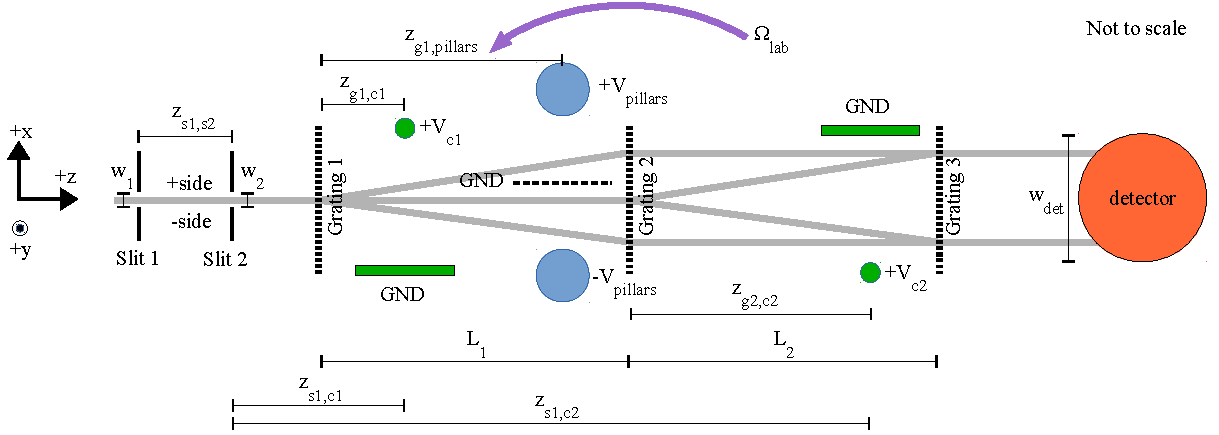
\includegraphics[width=\linewidth,keepaspectratio]{IFM_diagram1.pdf}
\caption{\label{IFMDiagram}(Color online) Diagram of the atom interferometry apparatus. The supersonic atom beam is collimated by two slits before entering the three-grating Mach-Zehnder interferometer. Due to the rotation of the Earth, the lab has a rotation rate about the vertical axis of $\Omega_{lab,y} = 38.88\mu$rad/s. }
\end{figure*}

\section{Apparatus Description and Error Analysis}

A schematic diagram of the three-grating Mach-Zehnder atom beam interferometer we use to make our measurements is shown in \figref{IFMDiagram}. We use a thermal, supersonic atom beam \cite{Scoles} seeded with a mixture of 85\% He and 15\% Ar gas that carries Cs, Rb, and K atoms at approximately 1800 m/s. 
The atoms pass through two collimating slits and then through three silicon nitride nano-gratings each with period $d_g = 100$ nm. We detect the atoms with a 100 $\mu$m-wide platinum wire Langmuir-Taylor detector \cite{Delhuille2002}.

The first two gratings form an interference pattern of period $d_g$ at the position of the third grating. By scanning the third grating in the $\pm x$ direction (as defined in \figref{IFMDiagram}), we can cycle between admitting and blocking the interference maxima and thus probe the interference pattern by observing changes in atom flux. In this manner, we observe interference fringes for Cs, Rb, and K using the same collimating slits, gratings, and detector.

We measure static polarizability $\alpha$ by polarizing the atoms with a non-uniform electric field created by two oppositely charged pillars parallel with the $y$ axis, indicated in blue in \figref{IFMDiagram}. The field shifts the phase of a single atom with velocity $v$ by an amount proportional to $\alpha/v^2$. We measure $v$ using phase choppers, which are charged wires parallel with the $y$ axis held near and parallel to grounded planes, indicated in green in \figref{IFMDiagram}. The phase choppers use the same field geometry as the pillars to apply a $\pm\pi$ phase shift to the atoms. In this section, we will explain how that field geometry induces phase shifts and how we use those fields to measure velocity and, thereby, polarizability. 

\subsection{Phase Shifts with Cylindrical Electrodes}
 
\begin{figure}
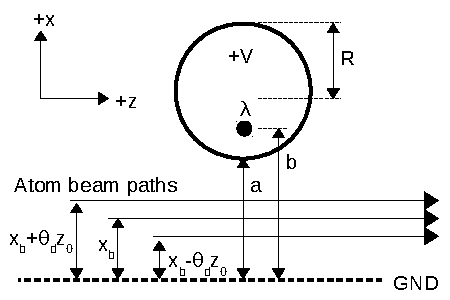
\includegraphics[width=\linewidth,keepaspectratio]{EDiagram1.pdf}
\caption{\label{EDiagram}(Color online) asdf}
\end{figure}

Our methods of measuring both the velocity distribution and polarizability involve applying a phase shift using non-uniform electric fields created by either a cylinder at voltage $V$ next to a grounded plane or two parallel cylinders at $\pm V$ forming an effective ground plane. 
Both configurations are described by the geometry shown in \figref{EDiagram}, and have fields given by
\begin{align}
	\vec{E} = \frac{\lambda}{\pi\epsilon_0}
	\left[	
		\frac{x-b}{(x-b)^2+z^2} - \frac{x+b}{(x+b)^2+z^2}
	\right] \hat{x} \nonumber \\
	+ 
	\left[	
		\frac{z}{(x-b)^2+z^2} - \frac{z}{(x+b)^2+z^2}
	\right] \hat{z}
	\label{EPillars}
\end{align}
The effective line charge density
\begin{align}
	\lambda = 2\pi\epsilon_0V\ln^{-1}
	\left(
		\frac{a+R+b}{a+R-b}
	\right)
	\label{lambda}
\end{align}
exists a distance $b = a\sqrt{1+2R/a}$ away from the ground plane, where $a$ is the distance between the ground plane and the closest cylinder edge, $R$ is the cylinders' radius, and $\hat{x}$ and $\hat{z}$ are shown in \figref{EDiagram}.

When an atom with polarizability $\alpha$ enters an electric field, it's energy shifts by $U_{Stark} = -\frac{1}{2}\alpha\abs{\vec{E}}^2$. We can use the WKB approximation (since $U_{Stark} \ll E_{kinetic}$) and the Residue Theorem to compute the total phase accumulated by an atom traveling along the beamline a distance $x_b$ away from the ground plane. Even though an atom in the beam may be misaligned by an angle of up to $10^{-3}$ with the fields' ground planes, we can approximate that atoms always travel parallel to the beamline: the effective path length through the field region grows as $1/\cos{\theta} \approx 1+\theta^2$, so a misalignment of $\theta = 10^{-3}$ should increase the phase by only one part in $10^6$, which is insignificant for our purposes. Therefore, the accumulated phase along the path is
\begin{align}
	\phi(v,x) = 
	\frac{1}{\hbar v} \int_{-\infty}^{\infty} \frac{1}{2} \alpha |\vec{E}|^2 dz =	
	\frac{\lambda^2 \alpha}{\pi \epsilon_0^2 \hbar v}
	\left( \frac{b}{b^2-x_b^2} \right)
	\label{accumPhasePillars}
\end{align}
where $v$ is the atom's velocity.

The different arms of the interferometer have different $x$ positions with respect to the electrodes, so the non-uniform electric field causes a differential phase shift. If the center of the field is a distance $z_0$ downstream of the first grating, for example, the atoms' possible paths are separated by a distance 
\begin{align}
	\theta_d z_0 = \frac{\lambda_{dB}}{d_g} z_0 = \frac{h}{mv}\frac{1}{d_g} z_0
	\label{pathSeparation}
\end{align}
where $\lambda_{dB}$ is the de Broglie wavelength. Paths closer to the effective line charges will acquire more total phase--thus the field causes a differential phase shift. The differential phase shifts for the interferometers on the $j=+1$ and $j=-1$ sides of the beamline (see \figref{IFMDiagram}) are
\begin{align}
	\Phi_{\vec{E},1}(v,x_b) = \phi(x_b+\theta_d z_0) - \phi(x_b) \nonumber \\
	\Phi_{\vec{E},-1}(v,x_b) = \phi(x_b) - \phi(x_b-\theta_d z_0)
	\label{deltaPhasePillars}
\end{align}
\figref{phaseShiftExample} shows an example of the interference fringes shifting due to an electric-field-induced differential phase shift.

\begin{figure}
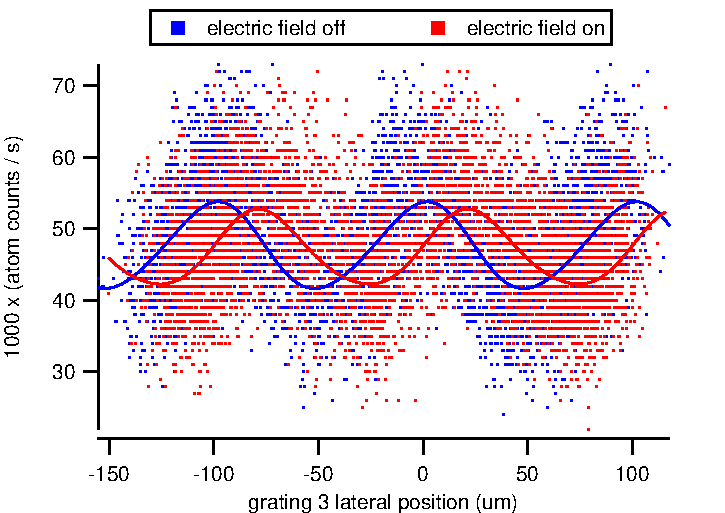
\includegraphics[width=\linewidth,keepaspectratio]{countsVsGratingPos_150420.pdf}
\caption{\label{phaseShiftExample}(Color online) An example of a differential phase shift. The blue and red Cs interference fringes were each observed by moving the third grating in the $\pm x$ direction for 5 seconds. A sine wave was fit to each interference pattern. This figure demonstrates the electric field moving the fringes by about 25 $\mu$m, or $d_g/4$, which corresponds to a $\pi/2$ differential phase shift.}
\end{figure}

\subsection{Velocity Measurement}

We model the atom beam's velocity distribution as a Gaussian distribution
\begin{align}
	P(v)dv = \frac{r}{v_0\sqrt{2\pi}}e^{-\frac{r^2(v-v_0)^2}{2v_0^2}}
	\label{PvelGaussian}
\end{align}
where $v_0$ is the mean velocity and $r = v_0/\sigma_v$ is a measure of the distribution's sharpness. When calculating the average contrast and phase of the ensemble of atoms, we must integrate over this velocity distribution. It is worth noting that the velocity distribution for a supersonic atom beam is actually
\begin{align}
	P(v)dv = \frac{1}{\sqrt{2\pi}v_0^4(r^{-1}+3r^{-3})}
	v^3
	e^{-\frac{r^2}{2}\left(\frac{v}{v_0}-1\right)^2}
	\label{PvelCubed}
\end{align}
However, both distributions are equally capable of parameterizing the typical velocity distributions of our atom beam. Since $v_0$ and $r$ are decoupled in the former and not in the latter, we choose to use the former for our data analysis because it simplifies discussion of the results. Using the latter does not change the polarizability result. 

To measure $v_0$ and $r$, we use phase choppers. Each phase chopper is a charged wire about 1 mm away from a physical ground plane. Chopper 1 is between the first two gratings and chopper 2 is a distance $z_{c1,c2} = (1269.3 \pm 0.25)$ mm downstream of chopper 1, between the last two gratings (see \figref{IFMDiagram}). The voltage on the wire and the distance between the beam and the ground plane are chosen such that chopper 1 shifts the ensemble's average phase by $+\pi$ and chopper 2 shifts the ensemble's average phase by $-\pi$. 

When we pulse the choppers on and off at frequency $f_c$, an atom may receive a net phase shift of $\pm\pi$ or $0$ depending on its velocity. Therefore, $v_0$, $r$, and $f_c$ determine the fraction of total atoms in the beam which receive a $\pm\pi$ phase shift. This fraction can be quantified by measuring contrast loss $C/C_{ref}$. To measure $v_0$ and $r$, we measure $C/C_{ref}$ vs $f_c$.

Using phase choppers allows us to measure $v_0$ and $r$ for Cs without needing to obtain resolved diffraction. In our earlier work, we measured $v_0$ and $r$ by scanning the detector's $x$ position to observe the diffraction pattern through grating 1. However, since the diffraction angle for Cs is so small, we would need a thinner detector wire and thinner collimating slits to resolve diffraction peaks, which would in turn reduce statistical precision.

We have identified a number of $v_0$-dependent systematic errors associated with phase chopper velocity distribution measurements. These errors must be quantified and reduced in order to measure polarizability ratios between atomic species that may typically run at different velocities.

In our previous work \cite{Hromada2014}, we documented the systematic errors that would appear if we were to not accurately know $\Delta L = L_1 - L_2$, where $L_1$ is the distance between gratings 1 and 2 and $L_2$ is the distance between gratings 2 and 3. There are two components to this error contribution. The first is that increasing $|\Delta L|$ shifts the interference fringes away from the beamline. We refer to this geometric fringe magnification as the separation phase, expressed as
\begin{align}
	\Phi_{sep,j} = \frac{2\pi}{d_g}
	\left(
		\theta_{inc} + \frac{j}{2}\theta_d
	\right) \Delta L
	\label{phiSep}
\end{align}
where $\theta_{inc}$ is the incident angle of a given atom with deBroglie wavelength $\lambda_{dB}$ on grating 1. The second component of the error is that, as $|\Delta L|$ increases, the longitudinal region at which the atoms' transverse coherence lengths overlap the most is moved away from grating 3, resulting in contrast loss \cite{Champenois1999,McMorran2008}. Furthermore, the electric fields, such as those created by the phase choppers, act as electrostatic lenses that magnify the interference fringes. This magnification also moves the maximal-overlap region longitudinally. Thus the choppers change the contrast simply by turning on, and changing the longitudinal location of the 3rd grating changes how the choppers modify the contrast. Because the ray optics model that we use to describe our interferometer does not assume finite transverse coherence lengths, we define $C_{env}$, the longitudinal contrast envelope which depends on $\Delta L$ and which electric fields are on.

We identified and reduced systematic error by modeling how the collimating slits define the beam's width and divergence and by considering the finite width of the detector, both of which determine how likely it is for atoms of a given velocity to be detected and thus contribute to a measurement of $v_0$. 
We accomplish this by integrating over possible trajectories through the slits (in addition to velocity), parameterized by x positions $x_1$ and $x_2$ from the centers of slits 1 and 2, in order to calculate the average contrast and phase of the atomic ensemble. We also define $D_j(x_1,x_2,v)$, the probability of an atom with velocity $v$ passing through the slits at positions $x_1$ and $x_2$ and diffracting to the $j$ side hitting the detector.
This new model also added elements to the error budget: the offset of the detector in the $x$ direction $\Delta x_{det}$ and the gratings' diffraction efficiencies determine how likely it is for atoms with certain velocities to be detected.

We find that as $\left|\Delta L\right|$ increases, the measured $v_0$ and $r$ become more dependent on the beam width, beam divergence, and detector width. Accordingly, we set $\Delta L = 0$ to reduce contributions to error in reported $v_0$ from other sources of uncertainty. We begin each day of measurements by setting $\Delta L$ to 0, eliminating the need to consider $\Phi_{sep}$. We know that if $\Phi_{sep}$ were nonzero, we would see the measured phase change as a function of $\Delta x_{det}$. We set $\Delta L = 0$ by finding the $\Delta L$ for which the measured phase no longer changes as a function of $\Delta x_{det}$ (see \cite{Hromada2014} for how we determined $C_{env}(t)$ experimentally).


If the interferometer grating bars are significantly non-vertical, it can become necessary to consider the phase shift induced by the component of gravitational acceleration in the plane of the interferometer, which is given by
\begin{align}
	\Phi_{accel} = \frac{\pi g\sin{\theta_g}(L_1+L_2)^2}{2d_g v^2}
	\label{phiAccel}
\end{align}
where $\theta_g$ is the tilt of the grating bars with respect to vertical. However, we eliminated the need to consider $\Phi_{accel}$ by rotating our grating bars so that they were sufficiently vertical. We measured $\theta_g$ to be $0 \pm 2 mrad$. Only if $|\theta_g| > ????$ would we need to add $\Phi_{accel}$ to our analysis.

Taking all these effects into account, our more complete model for contrast loss as a function of chopping frequency is
\begin{align}
	\frac{C}{C_{ref}}(f_c) = 
	\left|
		\frac{1}{2} \sum_{j=-1,1}
		f_c \int_{t=0}^{1/f_c} 
		\int_{x_1=w_1/2}^{w_1/2}
		\int_{x_2=w_2/2}^{w_2/2}
		\int_{v=0}^{\infty}           
		\right. \nonumber \\
		P(v)
		D_j(x_1, x_2, v)
		C_{env}(t)                   
		\nonumber \\ \times
		e^{i( \Phi_{c1,j}(v,x_1,x_2,t) + \Phi_{c2,j}(v,x_1,x_2,t-z_{c1,c2}/v) )}
		\nonumber \\ \times \left.
		e^{i( \Phi_{sep,j}(v,x_1,x_2) + \Phi_{accel}(v) + \Phi_{sag}(v) )}
		dv dx_{2} dx_{1} dt
	\right|
	\label{CvCF}
\end{align}
$\Phi_{ci,j}(v,x_1,x_2,t)$ is the differential phase shift induced by chopper $i$. $\Phi_{sag}(v)$ is the Sagnac phase, or the phase shift induced by the Earth's rotation \cite{Lenef1997,Jacquey2008}, and is given by
\begin{align}
	\Phi_{sag}(v) = \frac{4\pi L_2^2\Omega_{lab,y}}{d_g v}
	\label{phiSag}
\end{align}
The rotation rate of the interferometer about the vertical axis, $\Omega_{lab,y}$, is the product of the Earth's rotation rate and the sine of the lab's latitude. Not including the Sagnac phase in the analysis raises reported $r$ by about 1\%, which in turn causes $\alpha$ to be reported 0.25\% too high.

During times $t$ when the choppers are on, the chopper-induced phases $\Phi_{ci,j}(v,x_1,x_2)$ are adapted from \eqnref{deltaPhasePillars} and given by
\begin{align}
	\Phi_{c1,j}(v,x_1,x_2) = \frac{A_{c1}}{v}j \times \nonumber \\
	\left(
		\frac{1}{b_{c1}^2 -
			(x_{c1} + \frac{(x_2-x_1)}{z_{s1,s2}}z_{s1,c1} + x_2 + j\theta_d z_{g1,c1})^2
		}
		\right. \nonumber \\ - \left.
		\frac{1}{b_{c1}^2 -
			(x_{c1} + \frac{(x_2-x_1)}{z_{s1,s2}}z_{s1,c1} + x_2)^2
		}
	\right)
	\nonumber \\ 
	\nonumber \\	
	\Phi_{c2,j}(v,x_1,x_2) = \frac{A_{c1}}{v}j \times \nonumber \\
	\left(
		\frac{1}{b_{c2}^2 -
			(x_{c2} - \frac{(x_2-x_1)}{z_{s1,s2}}z_{s1,c2} - x_2 - j\theta_d z_{g1,g2})^2
		}
		\right. \nonumber \\ - \left.
		\frac{1}{b_{c2}^2 -
			(x_{c2} - \frac{(x_2-x_1)}{z_{s1,s2}}z_{s1,c2} - x_2 - j\theta_d z_{g2,c2})^2
		}
	\right)
	\label{phic1c2}
\end{align}
In the above equations, subscripts $sn$ and $gn$ on longitudinal distances $z$ represent collimating slit $n$ and grating $n$, respectively. $A_{c1}$ and $A_{c2}$ are undetermined constants that represent $\lambda_{ci}^2 \alpha / \pi \epsilon_0^2 \hbar$ from \eqnref{accumPhasePillars}. 

Instead of requiring accurate knowledge of the chopper voltages and geometries, we measure $A_{ci}$ indirectly. We turn chopper $i$ on and off with a 50 second period to observe the applied phase shift $\Delta\Phi = \Phi_{c1,on} - \Phi_{ref}$ and then solve for $A_{ci}$. When chopper $i$ is off, we observe the reference phase $\Phi_{ref}$ and reference contrast $C_{ref}$ given by 
\begin{align}
	C_{ref}e^{\Phi_{ref}} = 
		C_0e^{\Phi_0} \frac{1}{2} \sum_{j=-1,1}
		\int_{v=0}^{\infty}
		\int_{x_1=w_1/2}^{w_1/2}
		\int_{x_2=w_2/2}^{w_2/2} 
		\nonumber \\
		P(v) e^{\Phi_{sag}(v) + \Phi_{accel}(v) + \Phi_{sep,j}(v)} 
		dv
	\label{CPChoppersRef}
\end{align}
where $C_0$ is the contrast that would be observed in the absence of $\Phi_{sag}(v)$, $\Phi_{accel}(v)$, and $\Phi_{sep}(v)$, and $\Phi_0$ is an arbitrary phase constant. When chopper $i$ is on, we instead observe
\begin{align}
	C_{ci,on}e^{\Phi_{ci,on}} = 
		C_0e^{\Phi_0} \frac{1}{2} \sum_{j=-1,1}
		\int_{v=0}^{\infty}
		\int_{x_1=w_1/2}^{w_1/2}
		\int_{x_2=w_2/2}^{w_2/2} 
		\nonumber \\
		P(v) e^{\Phi_{ci,j}(v,x_1,x_2) + \Phi_{sag}(v) + \Phi_{accel}(v) + \Phi_{sep,j}(v)} 
		dv
	\label{CPChoppersOn}
\end{align}

\figref{CvCFExample} shows an example of a $C/C_{ref}$ vs $f_c$ measurement. 
For tutorial purposes, Eqns. \eqref{CvCF}, \eqref{CPChoppersRef}, and \eqref{CPChoppersOn} include $\Phi_{sep}$ and $\Phi_{accel}$ even though we have tuned our apparatus so that we need not include them in our analysis.

\begin{figure}
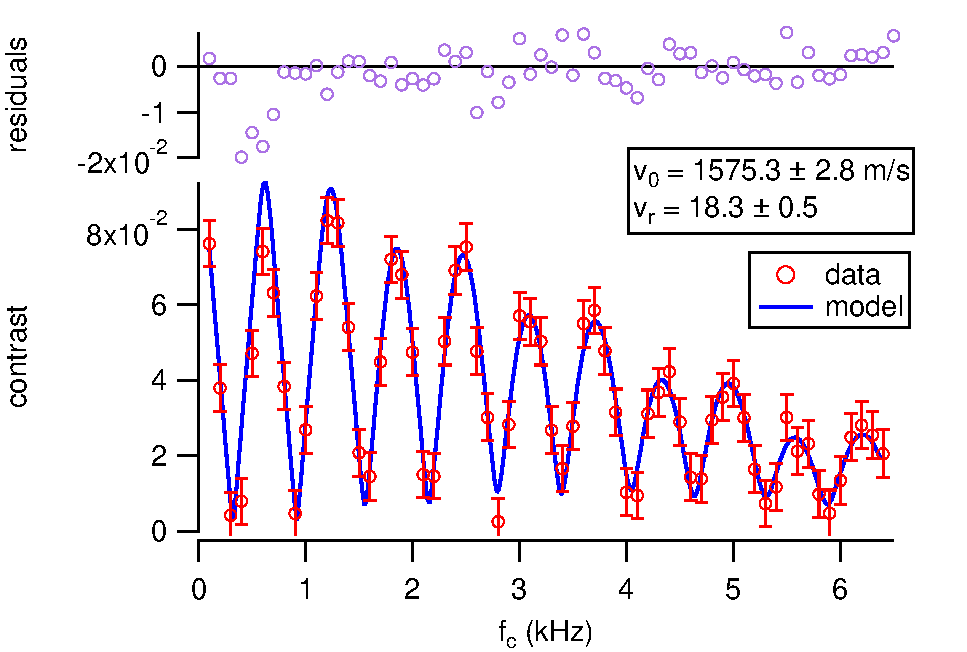
\includegraphics[width=\linewidth,keepaspectratio]{CvCF_150420_o.pdf}
\caption{\label{CvCFExample}(Color online) An example of a measurement of contrast loss vs. phase chopper frequency for a Cs beam. We fit a model to these data that has $v_0$ and $r$ as fit parameters in order to measure the velocity distribution.}
\end{figure}
	
The error budget for velocity distribution measurement is given in Table \ref{tableVelError}. The measured values of $v_0$ and $r$ also have statistical error in addition to uncertainty in the fit of measured $C/C_{ref}(f_c)$ to the model. Uncertainty in the measurement of $\Delta\Phi = \Phi_{c1,on} - \Phi_{ref}$ leads to uncertainty in $A_{ci}$, which in turn propagates forward as additional uncertainty in $v_0$ and $r$. The total statistical error in measured $v_0$ and $r$ is roughly $10\times$ larger than the total systematic error.

\begingroup
\begin{table}
\caption{\label{tableVelError}Systematic error budget for measurements of $v_0$ and $r$. Parameters $w_1$, $w_2$, and $w_{det}$ are the widths of collimating slits 1 and 2 and the detector. $a_{ci}$ is the width of phase chopper $i$, and $z_{c1,c2}$ is the longitudinal distance between choppers.}
\begin{center}
\begin{tabular}{l c c}
\hline\hline
Error Source & $\delta v_0/v_0 \times 1000$ & $\delta r/r \times 1000$ \\
\hline
$w_1 = (30 \pm 8) \mu\mathrm{m}$ 		& 0.05 & 1.0 \\
$w_2 = (40 \pm 8) \mu\mathrm{m}$ 		& 0.09 & 6.6 \\
$w_{det} = (100 \pm 10) \mu\mathrm{m}$ 		& 0.05 & 4.2 \\
$a_{c1} = (986 \pm 25) \mu\mathrm{m}$ 		& 0.005 & 0.1 \\
$a_{c2} = (893 \pm 25) \mu\mathrm{m}$ 		& 0.03 & 2.9 \\
$z_{c1,c2} = (1269.3 \pm 0.25) \mathrm{mm}$ 		& 0.20 & 0.1 \\
$C_{env} \mathrm{width} = (1.0 \pm 0.1) \mathrm{mm}$ 		& 0.06 & 2.7 \\
$\Delta x_{det} = (0 \pm 10) \mu\mathrm{m}$ 		& 0.006 & 0.15 \\
$\Delta L = (0 \pm 15) \mu\mathrm{m}$		& 0.098 & 6.0 \\
\hline
Total Sys. Error $\times 1000$ & $\sigv$ & $\sigr$ \\
\hline\hline
\end{tabular}
\end{center}
\end{table}
\endgroup

\subsection{Polarizability Measurement}

\begin{figure}
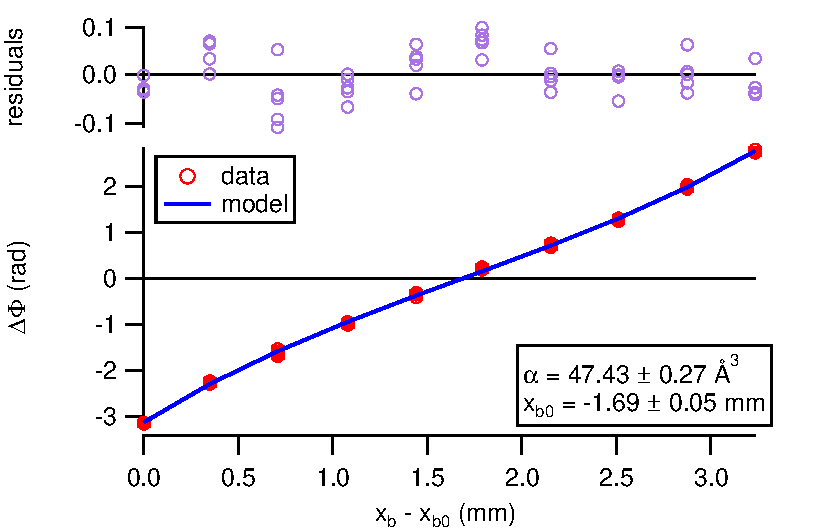
\includegraphics[width=\linewidth,keepaspectratio]{dPvMP_150327_q.pdf}
\caption{\label{dPvMPExample}(Color online) An example of a measurement of phase shift vs $x$ position of the pillars for a Rb beam. The fit parameters used to fit the model to these data are polarizability and the poles position at which the phase shift is null.}
\end{figure}

To measure the atoms' polarizability, we use two parallel, oppositely charged, $1/2$-inch-diameter pillars mounted to a single, rigid support structure. The pillars are mounted so that a $(3999.7 \pm 1.0)\mu$m gap exists between them. A motor moves the support structure in the $\pm x$ direction, and a length gauge monitor's the structure's $x$ position. We scan the assembly across the beam so that the beam traverses the gap between the pillars, turning the field on and off as it scans, to observe the phase shift $\Delta\Phi = \Phi_{pillars,on} - \Phi_{ref}$ applied by the pillars as a function $x_b$ (see an example in \figref{dPvMPExample}). $\Phi_{ref}$ is once again the reference phase and contrast observed when there are no polarizing electric fields present.
When the pillars are on, we instead observe
\begin{align}
	C_{\vec{E}\textit{ on}}e^{\Phi_{\vec{E}\textit{ on}}} = 
		C_0e^{\Phi_0}		
		\frac{1}{2} \sum_{j=-1,1}
		\int_{v=0}^{\infty} P(v) \nonumber \\ \times
		e^{
			\Phi_{\vec{E},j}(v,x_b) + 
			\Phi_{sag}(v) + \Phi_{accel}(v) + \Phi_{sep,j}(v)
		} 
		dv
	\label{CPPolesEOn}
\end{align}
We fit a model to $\Delta\Phi = \Phi_{pillars,on} - \Phi_{ref}$ as shown in \figref{dPvMPExample}, the fit parameters of which are $\alpha$ and the pillars position for which the phase shift is null. Because $\Delta\Phi$ vs pillars position is very linear near the zero crossing, we can determine that zero crossing to very high precision. 
This changes a previously significant systematic error, associated with measuring the distance between the beam and the physical ground plane, into an insignificant statistical error.

\begingroup
\begin{table}
\caption{\label{tablePolError}Error budget for polarizability measurements. The uncertainties in knowledge of $v_0$ and $r$ are propagated forward from Table \ref{tableVelError}.}
\begin{center}
\begin{tabular}{l c c}
\hline\hline
Error Source & $\delta\alpha/\alpha \times 1000$ \\
\hline
$d_g = (100.0 \pm 0.1) \mathrm{nm}$ 		& 1 \\
$V_{pillars}: \delta V/V = 0.0005$ 		& 1 \\
$a_{pillars} = (3999.7 \pm 1.0) \mu\mathrm{m}$ 		& 0.7 \\
$R_{pillars} = (6350 \pm 1) \mu\mathrm{m}$ 		& 0.07 \\
$v_0: \delta v_0/v_0 = \sigv$		& 0.56 \\
$r: \delta r/r = \sigr$ 		& 0.28 \\
$z_{g1,pillars} = (833.5 \pm 0.25) \mathrm{mm}$ 		& 0.6 \\
dimer fraction $ < 0.02$ 		& 0.46 \\
$\Delta L = (0 \pm 15) \mu\mathrm{m}$ 		& 0.16 \\
\hline
Total Sys. Err. $\times 1000$ & 1.9 \\
\hline\hline
\end{tabular}
\end{center}
\end{table}
\endgroup

The error budget for the absolute polarizability measurements is given in Table \ref{tablePolError}. The only new terms are uncertainty in $\Delta L$ because of separation phase (\eqnref{phiSep}), and uncertainty in grating tilt because of acceleration phase (\eqnref{phiAccel}).

We constructed the new pillars using steel rods, the widths of which were accurately known to $1 \mu \text{m}$. This reduced the contribution to $\delta\alpha/\alpha$ from uncertainty in pillars radius by about a factor of 10. The new pillars have a virtual ground plane between then rather than consisting of one pillar and a physical ground plane as they did in our previous work; being able to measure the phase shift with the beam on both sides of the ground plane makes it unnecessary to consider $\Phi_{sag}$. 

We reduced some error contributions simply by measuring the apparatus geometry more carefully. We reduced $\delta\alpha/\alpha$ due to uncertainty in the pillars' voltage by a factor of 3 by independently calibrating our voltage supplies. We also reduced $\delta\alpha/\alpha$ due to uncertainty in distance between the pillars and the effective ground plane by sweeping the pillars across the atom beam and observing how far the pillars traveled between points at which the atom beam half-eclipsed each pillar. We were able to measure the distance between the first grating and the pillars to 1/4 mm accuracy rather than 2 mm accuracy. 

It is important to note that measurements of $\alpha$ are not significantly affected by whether or not we consider $\Phi_{accel}$ in our polarizability analysis or in our velocity distribution analysis because the grating bars are sufficiently vertical. Therefore, $\Phi_{sag}$, $\Phi_{accel}$, and $\Phi_{sep}$ are included in \eqnref{CPPolesEOn} for tutorial purposes only--our result is unaffected if we remove them.

Additionally, we found that modeling the beam's thickness and divergence was unnecessary for analysis of polarizability data if $\Delta L = 0$ and becomes increasingly important as $|\Delta L|$ increases. Because we keep $\Delta L$ close to 0, we find our reported results do not change if we model the beam's thickness and divergence.

Finally, we report that considering second order diffraction in our model of the interferometer does not change $v$ by more than 0.05 ppt, $r$ by 2 ppt, and $\alpha$ by 0.1 ppt. This is primarily because the fraction of atoms in those interferometer paths is so small. Also, second-order diffraction angles are small enough so that the atoms hit the detector, then they are not sufficiently separated from the first-order interferometer paths.

\subsection{Data Analysis}

\begin{figure*}
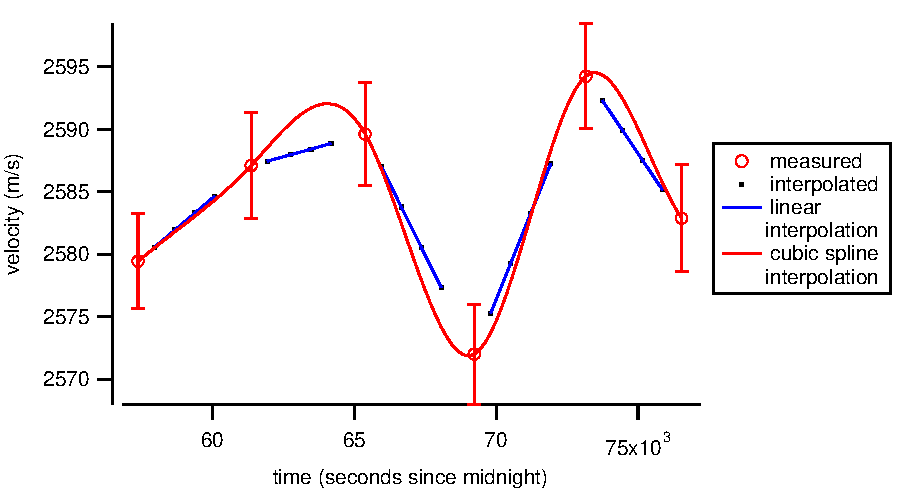
\includegraphics[width=0.49\linewidth,keepaspectratio]{velVsTime_150212.pdf}
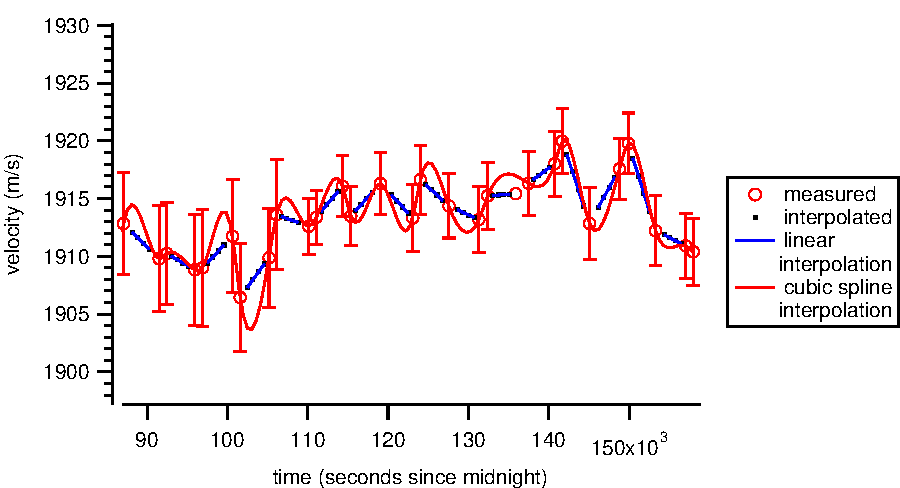
\includegraphics[width=0.49\linewidth,keepaspectratio]{velVsTime_150413.pdf}
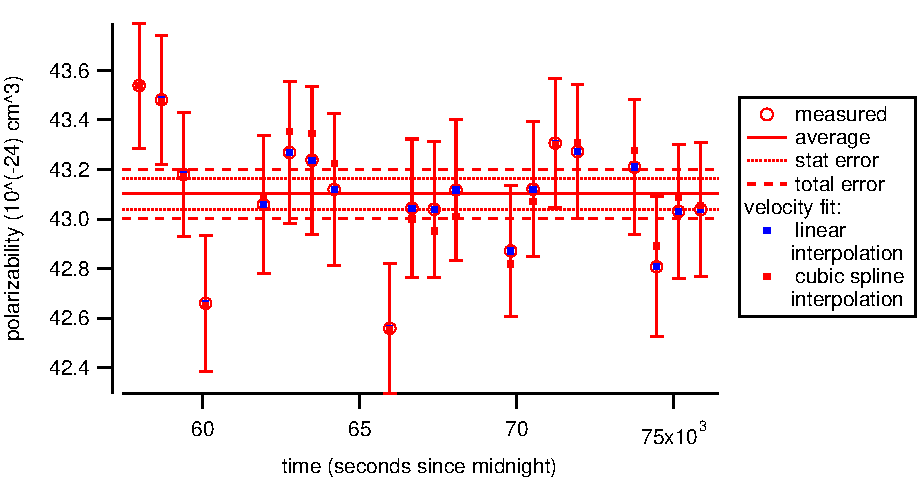
\includegraphics[width=0.49\linewidth,keepaspectratio]{polVsTime_150212.pdf}
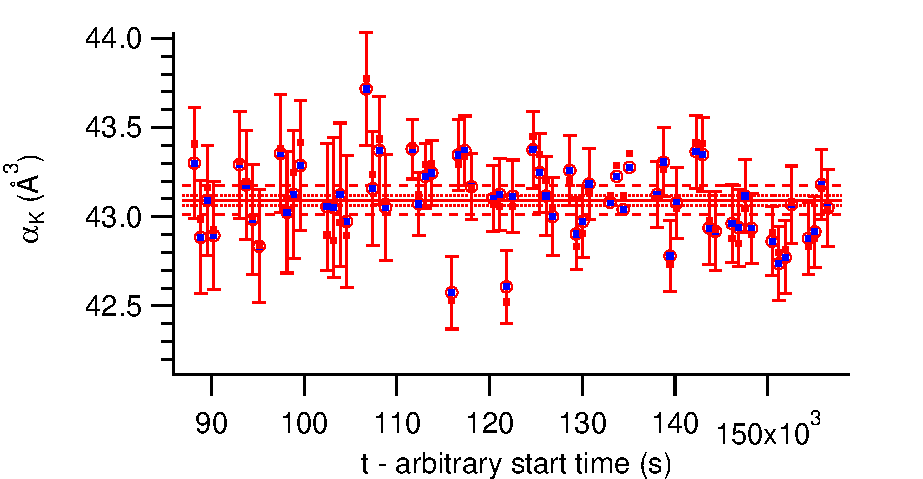
\includegraphics[width=0.49\linewidth,keepaspectratio]{polVsTime_150413.pdf}
\caption{\label{velPolVsTimeExample}(Color online) The results of $v_0$ (top) and $\ak$ (bottom) measurements taken during two different days (left and right). Both linear and cubic spline interpolations between $v_0$ measurements are reasonable, and higher differences between the two interpolations during $\ak$ measurements increase the error bars on said measurements. For these data, we chose to use linear interpolation because we believe it more accurately represents $v_0$ vs $t$--the cubic spline interpolation sometimes gains too much curviture, especially when back-to-back velocity measurements, such as those in the top-left, yield results that differ by an error bar. The red dots on the bottom graphs show what the measured $\ak$ would be if we were to use cubic spline interpolation instead. The top graphs show some typical structures that occur in $v_0$ vs time. This figure also demonstrates how we obtain the same $\ak$ for very different velocities.}
\end{figure*}

\begingroup
\begin{table}
\caption{\label{schedule}A typical sequence of measurements during a day of data acquisition. The $+x$ direction is arbitrarily chosen--the important aspect is that we spend an equal amount of time scanning the pillars in each direction so as to minimize possible systematic errors. This sequence of eight measurements is repeated for as long as we choose to acquire data. We end the data acquisition by repeating the first four measurements.}
\begin{center}
\begin{tabular}{l}
\hline
contrast vs chopping freq. \\
chopper 1 phase \\
chopper 2 phase \\
contrast vs chopping freq. \\
$\Delta\Phi$ vs pillars position ($+x$ direction) \\
$\Delta\Phi$ vs pillars position ($-x$ direction) \\
$\Delta\Phi$ vs pillars position ($+x$ direction) \\
$\Delta\Phi$ vs pillars position ($-x$ direction) \\
\hline
\end{tabular}
\end{center}
\end{table}
\endgroup

A typical sequence of measurements is shown in Table \ref{schedule}.
We measure the velocity distribution twice between every four scans of the pillars across the beam, and calibrate the phase choppers between each pair of velocity measurements.
We interpolate the velocity distribution between measurements to estimate it for each pillars scan. The error bars on each interpolated $v_0$ and $r$ value are due to the error bars on neighboring measurements and the different ways we believe $v_0$ and $r$ might be reasonably interpolated. For example, we believe linear and cubic spline interpolations are reasonable, so the error bars at a given time take into account the differences between those interpolations--a larger difference between reasonable interpolations leads to larger error bars on interpolated values. That error is then propagated forward and combined with the statistical error of the fit to $\Delta\Phi$ vs $x_b$ to determine the error bars on the polarizability measurements. \figref{velPolVsTimeExample} shows an example of interpolations between $v_0$ measurements at the times of various pillars scans.

\section{Results}

Table \ref{tableAbs} shows our absolute measurements of Cs, Rb, and K polarizability and their statistical and systematic errors. The error reported is the standard error of the mean. Table \ref{tableAbs} also shows $\chi^2/(\text{degree of freedom})$ for each measurement; we can see that we are operating near the shot-noise limit. 

\begingroup
\begin{table}
\caption{\label{tableAbs}Absolute measurements of Cs, Rb, and K static, ground-state polarizabilities.}
\begin{center}
\begin{tabular}{l l l l l}
\hline\hline
Atom & avg $v_0$ (m/s) & avg $r$ & $\alpha$(stat.)(sys.) ($\AA^2$) & $\chi^2/DoF$ \\
\hline
Cs & 1587 & 21 & $\polCs$ & 1.02 \\
Rb & 1891 & 24 & $\polRb$ & 1.05 \\
K  & 2118 & 14 & $\polK$ & 1.26 \\
\hline\hline
\end{tabular}
\end{center}
\end{table}
\endgroup

Table \ref{tableRatio} shows our ratio measurement results. Because we used the same apparatus for each absolute measurement, we can say that the systematic errors mentioned previously do not contribute to the ratio measurement errors. This is important because even if a systematic error causes our absolute measurements to be incorrect, our ratios should still be reliable. \textit{This statement does not jibe with the earlier statement that some systematic errors are velocity-dependent. I'm looking into this now} 

\begingroup
\begin{table}
\caption{\label{tableRatio}Ratio measurements of Cs, Rb, and K static, ground-state polarizabilities.}
\begin{center}
\begin{tabular}{l l}
\hline\hline
Atoms & ratio(stat.) \\
\hline
Cs:Rb & $\ratCsRb$ \\
Cs:K  & $\ratCsK$ \\
Rb:K  & $\ratRbK$ \\
\hline\hline
\end{tabular}
\end{center}
\end{table}
\endgroup

\section{Comparisons with other work}

\begin{figure*}
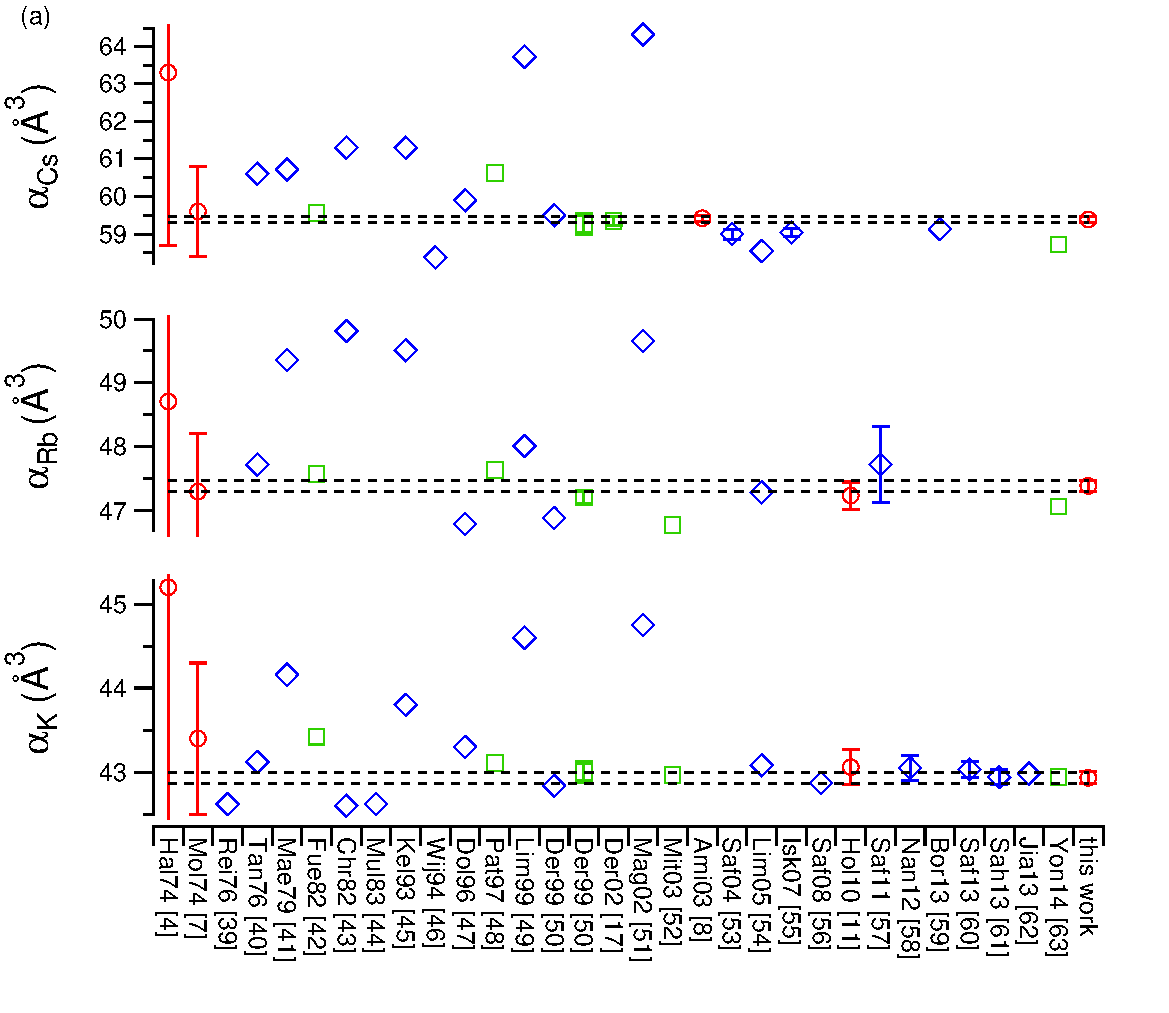
\includegraphics[width=0.59\linewidth,keepaspectratio]{displayAbsComps.pdf}
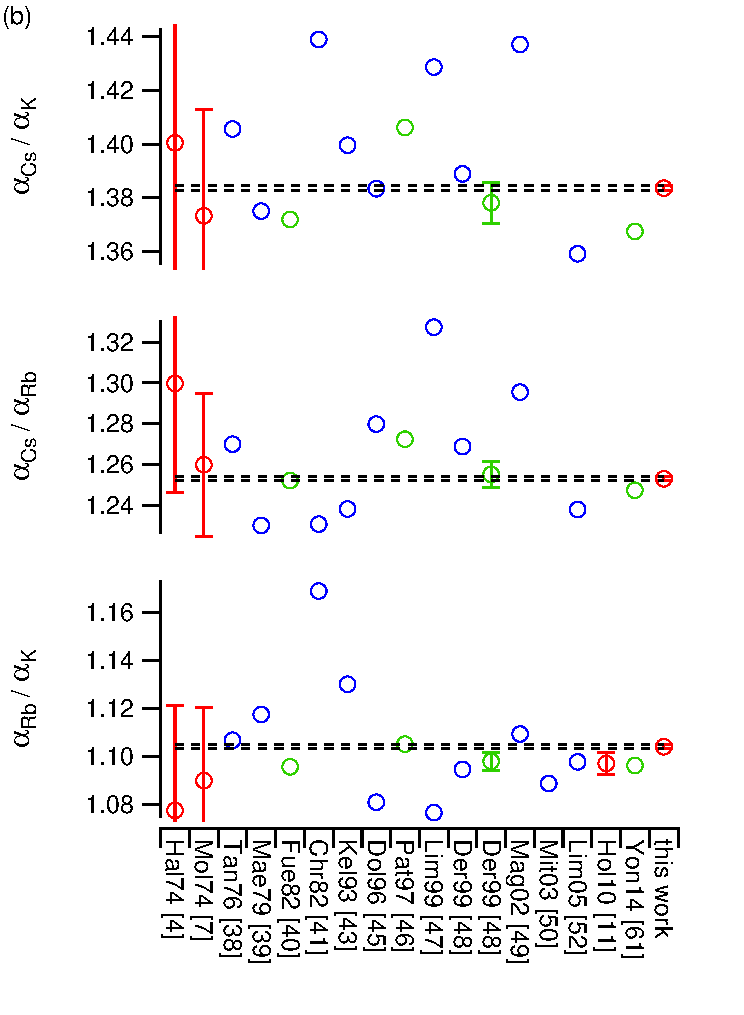
\includegraphics[width=0.4\linewidth,keepaspectratio]{displayRatComps.pdf}

\includegraphics[width=0.55\linewidth,keepaspectratio]{displayCompsLegend.pdf}
\caption{\label{comparisons}(Color online) Our absolute measurements (left) and ratio measurements (right) compared with other measurements, \textit{ab initio} calculations, and semi-empirical calculations 
\cite{
Molof1974,Hall1974,Tang1976,Reinsch1976,Kutzelnigg1978,
Christiansen1982,Fuentealba1999,Muller1984,Kello1993,VanWijngaarden1994,
Dolg1996,Patil1997,Derevianko1998,Magnier2002,Derevianko2001,
Amini2003,Lim2005,Safronova2008,Holmgren2010,Nandy2012,
Jiang2013,Sahoo2013,Safronova2013,Borschevsky2013}.
The references are represented on the x-axis by the first three letters of the first author's last name followed by the year of publication. Reference Der99 used experimentally-determined electric dipole matrix elements, while reference Pat97 used experimentally-determined energy levels \cite{Derevianko1998,Patil1997}}.
\end{figure*}

\begin{figure}
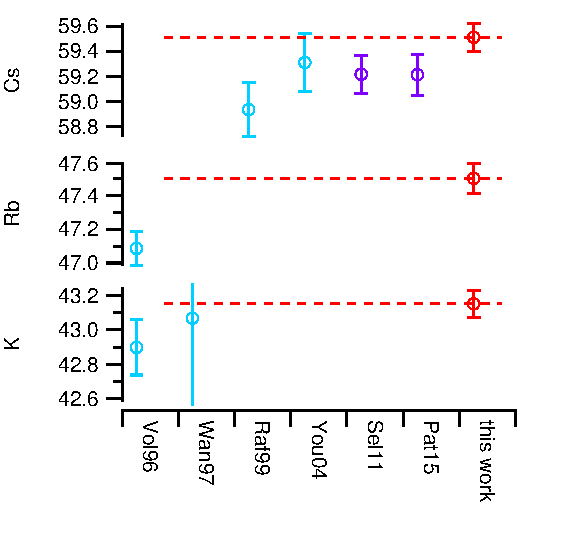
\includegraphics[width=\linewidth,keepaspectratio]{displayLifeComps.pdf}
\caption{\label{comparisonsLifetimes}(Color online) Our measurements (red) are compared with polarizabilities calculated using experimentally measured lifetimes \cite{Young1994,Volz2006,Wang1997,Rafac1999,Sell2011,Patterson2015}. Light blue points were calculated using both $Ns-Np_{1/2}$ and $Ns-Np_{3/2}$ lifetimes, while dark purple points were calculated using $Ns-Np_{3/2}$ lifetimes and the $Ns-Np_{3/2}$:$Ns-Np_{1/2}$ ratio provided by Young \etal \cite{Young1994}}
\end{figure}

\figref{comparisons} compares our polarizability measurements with theoretical calculations, semi-empirical calculations, and experimental measurements subsequent to and including Molof \etal's and Hall \etal's 1974 measurements \cite{Molof1974,Hall1974}. Our absolute measurements are consistent with all previous absolute measurements, though our Cs measurement is only barely consistent with Amini and Gould's. As a self-consistency check: our measurements are systematically higher, though still statistically consistent with, our lab's previous measurements \cite{Holmgren2010}. At present, we don't have an explanation for these almost-discrepancies. We acknowledge the possibility of a systematic error in our experiment we are as of yet unaware of, and we hope to calibrate our measurements in the future by measuring a well-known polarizability, such as that of lithium or metastable helium.

\figref{comparisons} also compares our ratios to other theoretical, semi-empirical, and experimental ratios. Our ratios are also consistent with all previous measurements.

Additionally, we can compare our measurements to polarizabilities calculated using recent high-precision measurements of state lifetimes. For an atom in state $i$, the polarizability can be written in terms of Einstein A coefficients as
\begin{align}
	\alpha_i = \frac{3c^3}{2} \sum_{k\neq i} 
	\frac{A_{ki}}{\omega_{ik}^4} \frac{g_k}{3g_i}
	+ \alpha_{core}
	+ \alpha_{tail}
	\label{polFromLifetimes}
\end{align}
where $\omega_{ik}$ is the transition frequency between states $i$ and $k$ and $g_n = 2J_n+1$ is the degeneracy factor for state $n$. In our case, state $i$ is the ground state. $\alpha_{core}$ is the polarizability of the core electrons, and $\alpha_{tail}$ approximates all the terms not explicitly included in the sum; we will only be using measured lifetimes for $Ns-Np$ transitions.
We use Lim \etal's calculated core polarizabilities of 
$\alpha_{core,\mathrm{K}} = 0.818(6) \AA^3$, 
$\alpha_{core,\mathrm{Rb}} = 1.350(6) \AA^3$, and 
$\alpha_{core,\mathrm{Cs}} = 2.341(15) \AA^3$ \cite{Lim2002}. 
Furthermore, Derevianko and Porsev calculated that 
$\alpha_{tail,\mathrm{Cs}} = 0.162 \AA^3$ {Derevianko2001}. Because we lack values for $\alpha_{tail,\mathrm{Rb}}$ and $\alpha_{tail,\mathrm{K}}$ and because $\alpha_{tail,\mathrm{Cs}}$ only accounts for 0.27\% of $\acs$, we can approximate for these purposes that $\alpha_{tail}$ accounts for 0.27\% of $\alpha$ for Rb and K as well. The $\omega_{0k}$ values are calculated using transition wavelengths reported by NIST \cite{NIST}. 

\figref{comparisonsLifetimes} compares our measurements with these lifetime-based results. Our measurements are significantly higher than most of the values based on recent lifetime measurements. Because the lifetime measurements were all made by different people using different experimental methods, these discrepancies strongly suggest that our absolute polarizability measurements are too high and require calibration.

\section{Outlook}

We are currently exploring ways to measure the polarizability of metastable He, the polarizability of which can be easily calculated. By measuring $\acs:\alpha_{He*}$, we could report an absolute measurement of $\acs$ with uncertainty comparable to that of the ratios reported here for the benefit of PNC research and as a calibration of the measurements presented in this work.

We are also exploring electron-impact ionization schemes for atom detection, which would allow us to detect a much broader range of atoms and molecules. Our Langmuir-Taylor only allows us to detect alkali metals and some alkaline-Earth metals. Installing a new, "universal" detector would allow us to broaden the scope of atom interferometry as a precision measurement tool. 

This work is supported by NSF Grant No. 1306308 and a NIST PMG. M.D.G. and R.T. are grateful for NSF GRFP Grant No. DGE-1143953 for support. 


%\bibliography{references}
\bibliography{library}

\end{document}  